\documentclass[10pt]{article}


\usepackage[utf8]{inputenc}

\usepackage{hyperref}
\usepackage{graphicx}
\usepackage{amssymb}
\usepackage{color}
\usepackage{listings}
\usepackage{tikz}
\usepackage{verbatim}
\usepackage{theorem}



\begin{document}

\title{ML4PG: Machine learning for Proof General}
\author{J\'onathan Heras and Ekaterina Komendantskaya\\
\{jonathanheras,katya\}@computing.dundee.ac.uk}
 \maketitle
 
 
 
\tableofcontents 
 

\section{Using ML4PG}


To illustrate the use of ML4PG, we will use the file \verb"ml4pg.v" which can be find in the same folder of this manual.
This file contains various lemmas about natural numbers and lists.

\subsection{Getting started}

Open the file \verb"ml4pg.v" using emacs. The Proof General interface is the usual one, but it includes a new option in the Coq menu
called ML4PG.

\begin{figure}
 \centering
 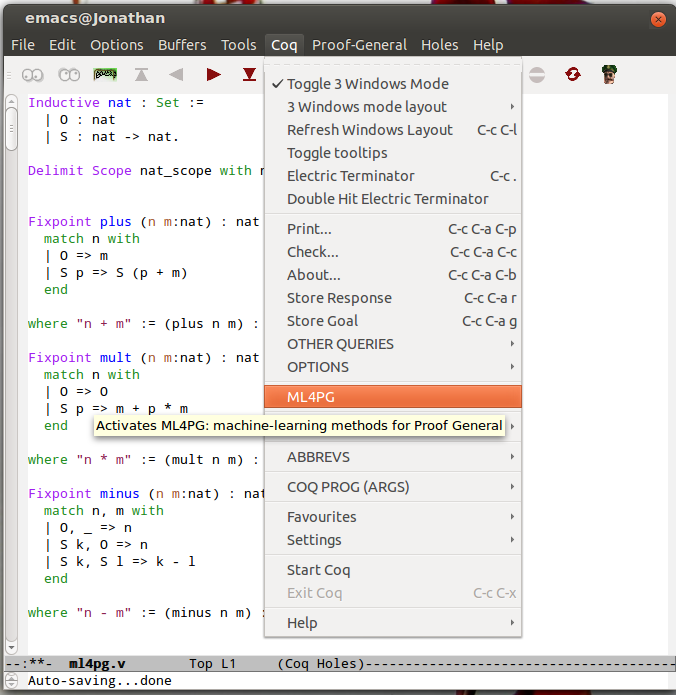
\includegraphics[scale=0.4]{images/fig1pg.png}
 \caption{Proof General with the ML4PG option.}\label{fig1}
\end{figure}

If you select this option, the interface asks you if you are developing your proofs using the plain Coq style or the SSReflect style, in this case we select the Coq mode (c). 
Subsequently, the interface asks you if you want to extract the information associated with the lemmas which have been previously developed in this library. In this case,
we select no (c). Once that this is done, the Proof General interface is extended with a new menu called \emph{Statistics} and two buttons, see Figure~\ref{fig3}.

\begin{figure}
 \centering
 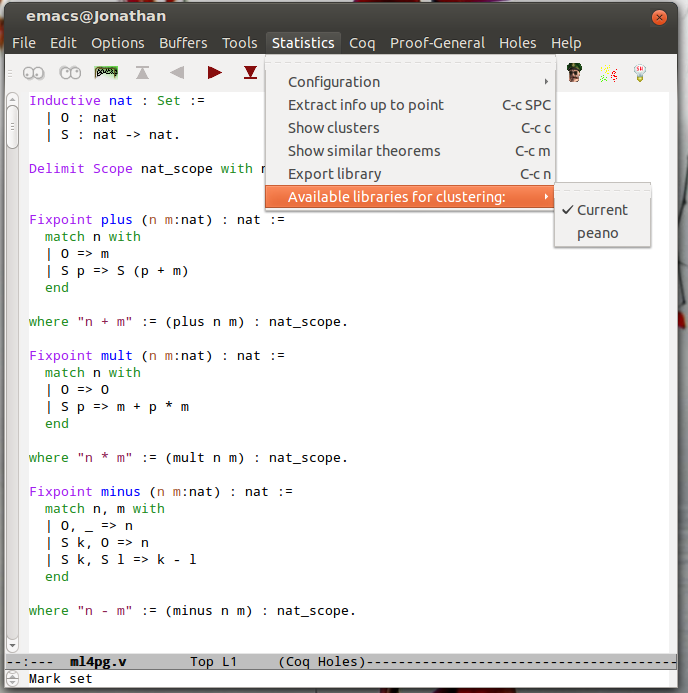
\includegraphics[scale=0.4]{images/fig3.png}
 \caption{ML4PG interface with all the options active.}\label{fig3}
\end{figure}


\subsection{Extracting feature vectors}

Feature vectors can be extracted in two different ways:

\begin{itemize}
 \item During the development of the proofs. To this aim, you have to use the shortcut Ctrl-C Ctrl-M to process the next proof command.
 \item Several proofs at the same time. If you want to extract the feature vectors of several proofs, go to the last proof and use the shortcut Ctrl-C Space. 
       You can also use the \emph{Extract info up to point} option of the statistics menu. 
\end{itemize}

Go to the end of \verb"emacs ml4pg.v" file; there, you can see two unfinished proofs: \verb"M3_3b" and \verb"aux7_bis". Put the cursor at the end of 
the proof of Lemma \verb"andb_false_r" and use the shortcut Ctrl-C Space or the \emph{Extract info up to point} option of the statistics menu. In this 
way the information associated with each proof will be extracted and you will be able to use it to obtain proof clusters (groups of similar proofs).

Now, let us explain the functionality of the options included in the Statistics menu. 

\subsection{Configuration menu}

The different options to configure the Machine-learning environments were detailed in~\cite{KHG12}. All those options can be accessed from the Configuration 
submenu of the Statistics menu, see Figure~\ref{fig3}. 



\paragraph{Algorithms:}

The user can select different algorithms to obtain proof similarities (all of them behave similar, see~\cite{HK13}).
ML4PG offers different algorithms, see Figure~\ref{algorithms}. 

In the case of MATLAB; there are three algorithms available: K-means and Gaussian. In the case of Weka, the algorithms 
which are available are: K-means, EM and FarthestFirst. 

\begin{figure}
 \centering
 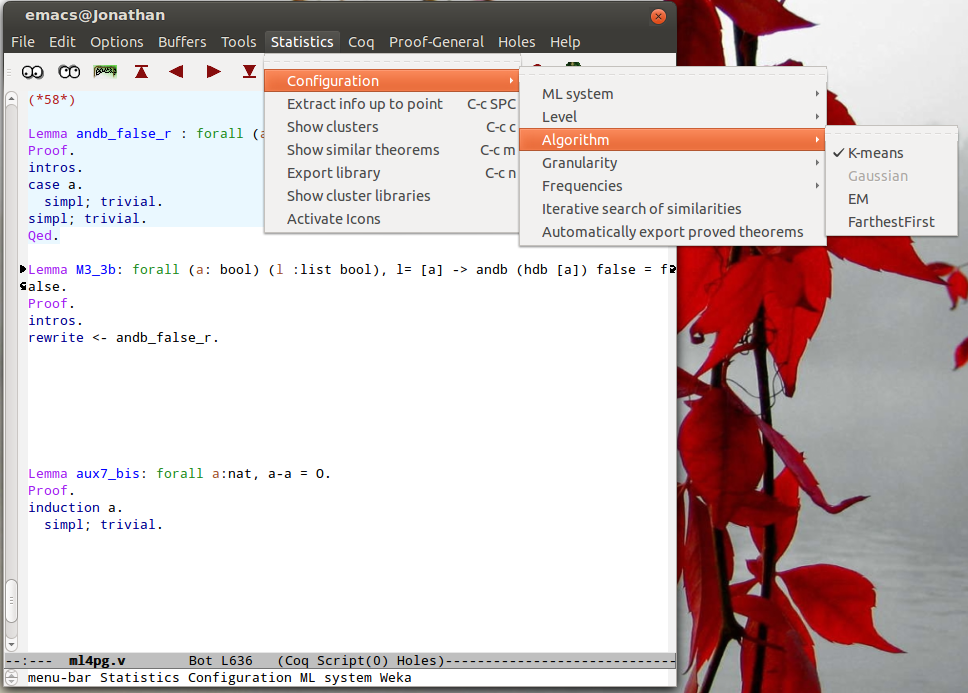
\includegraphics[scale=0.4]{images/algorithm2.png}
 \caption{The ML algorithms menu.}\label{algorithms}
\end{figure}

\paragraph{Granularity:}

In the machine learning literature, there exists a number of heuristics to determine this optimal number of clusters.
We used them as an inspiration to formulate our own algorithm for ML4PG, tailored
to the interactive proofs. It takes into consideration the size of the proof library and an auxiliary parameter 
 -- called granularity. This parameter is used to calculate the optimal number of
proof clusters, the process to calculate this optimal number was described in~\cite{KHG12}. The user decides the 
granularity in ML4PG menu (see Figure~\ref{granularity}), by selecting a value between 1 and 5, where 1 stands for a
low granularity (producing big and general clusters) and 5 stands for a high granularity (producing small
and precise clusters). 


\begin{figure}
 \centering
 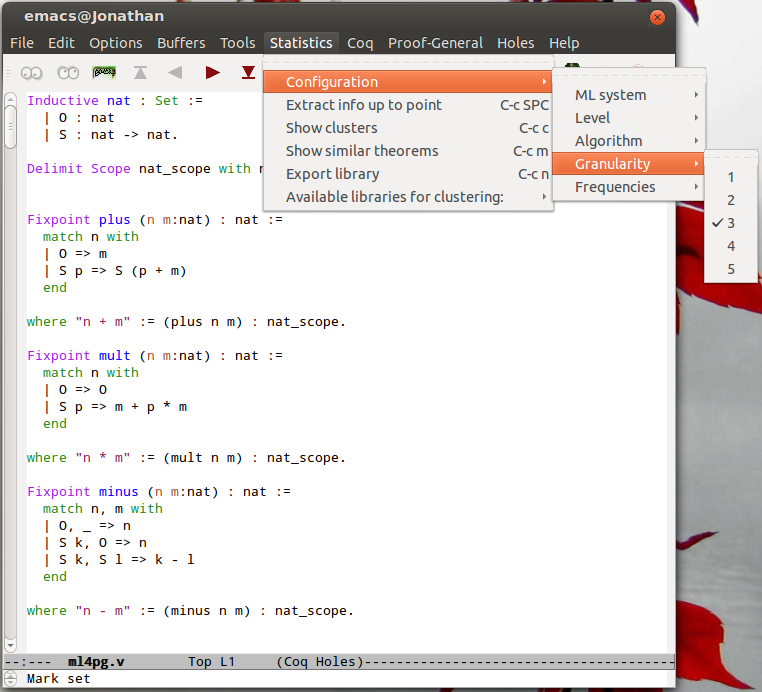
\includegraphics[scale=0.4]{images/granularity.png}
 \caption{ML4PG granularity menu.}\label{granularity}
\end{figure}



\paragraph{Frequencies:}

Clustering techniques divide data into n groups of similar objects (called clusters), where the value of
n is a ``learning'' parameter provided by the user together with other inputs to the clustering algorithms.
Increasing the value of n means that the algorithm will try to separate objects into more classes, and, as a
consequence, each cluster will contain examples with higher correlation. The frequencies of clusters can
serve for analysis of their reliability. Results of one run of a clustering algorithm may differ from another,
even on the same data set. This is due to the fact that clustering algorithms randomly choose examples
to start from, and then, form clusters relative to those examples. However, it may happen that certain
clusters are found repeatedly – and frequently – in different runs; then, we can use these frequencies to
determine the reliable clusters. The frequencies can be determined using the threshold presented in Figure~\ref{frequencies},
a detailed description of this parameter was given in~\cite{KHG12}.


\begin{figure}
 \centering
 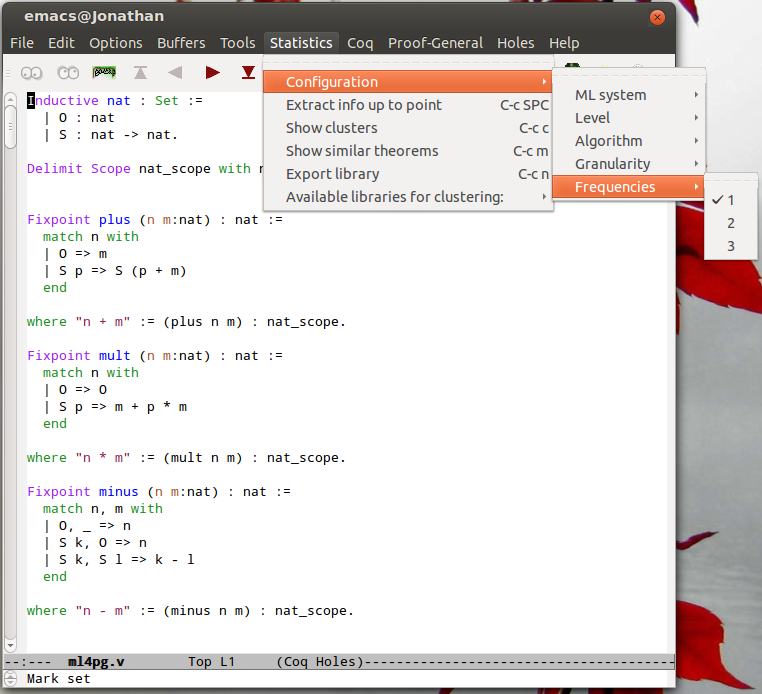
\includegraphics[scale=0.4]{images/frequencies.png}
 \caption{ML4PG frequencies menu.}\label{frequencies}
\end{figure}


\subsection{Show clusters}

The option \emph{Show Clusters} of the Statistics menu shows clusters when a library is clustered
irrespective of the current proof goal. An example using the \verb"ml4pg.v" library with the options:

\begin{itemize}
 \item Algorithm: K-means,
 \item Granularity: 3,
 \item Frequencies: 1.
\end{itemize}

\noindent is shown in Figure~\ref{clusters1}.

\begin{figure}
 \centering
 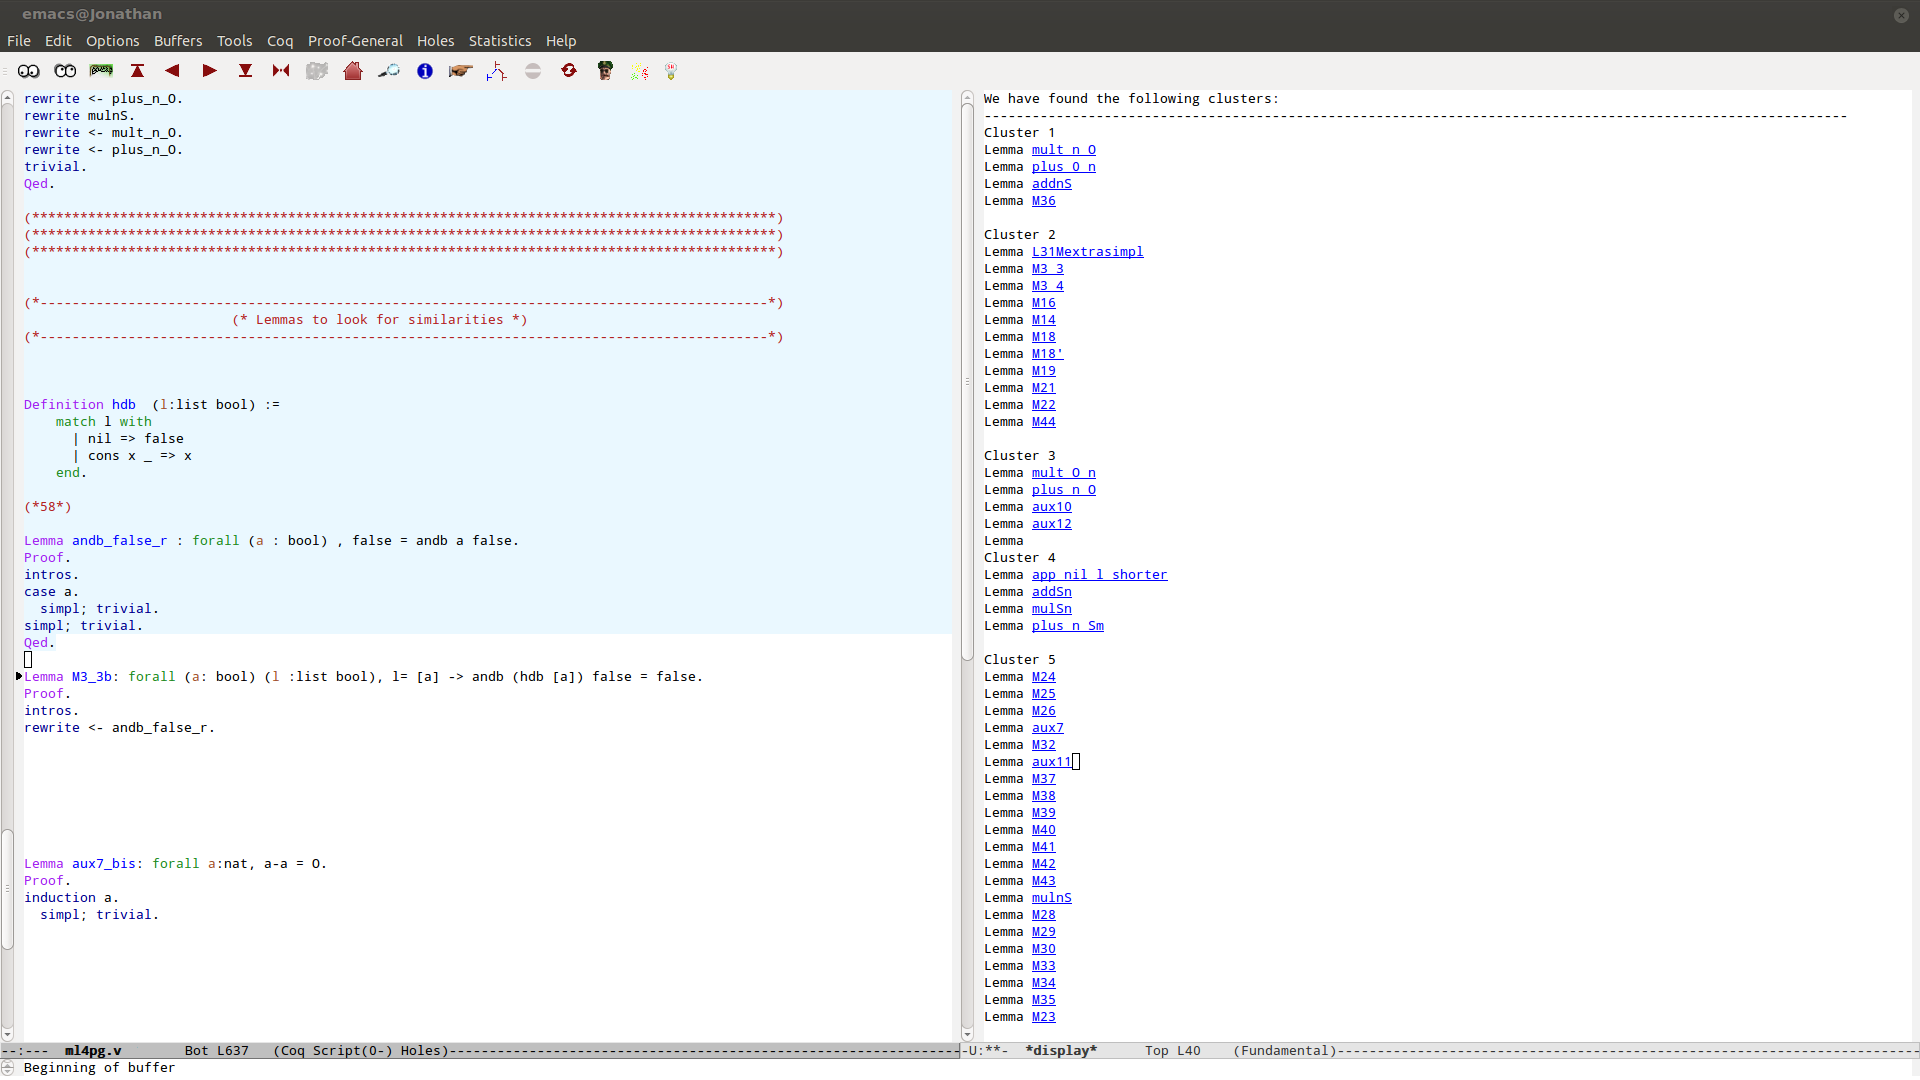
\includegraphics[scale=0.23]{images/clusters1pg.png}
 \caption{Clusters for the ml4pg library. The Proof General window has been split into two windows positioned side by
side: the left one keeps the current proof script, and the right one shows the clusters. If the user clicks
on the name of a theorem showed in the right screen, such a window is split horizontally and a brief description of the selected
theorem is shown.}\label{clusters1}
\end{figure}

This functionality can also invoked using the second right most button of the Proof General toolbar.

\subsection{Show similar theorems}

The example above shows one mode of working with ML4PG: that is, when a library is clustered
irrespective of the current proof goal. However, it may be useful to use this technology to aid the interactive
proof development. In which case, we can cluster libraries relative to a few initial proof steps for the
current proof goal. An example using the \verb"ml4pg.v" library with the options:

\begin{itemize}
 \item Algorithm: FarthestFirst,
 \item Granularity: 2,
 \item Frequencies: 2.
\end{itemize}

\noindent and with the few steps included about the proof of \verb"M3_3b" is shown in Figure~\ref{clusters2}.


\begin{figure}
 \centering
 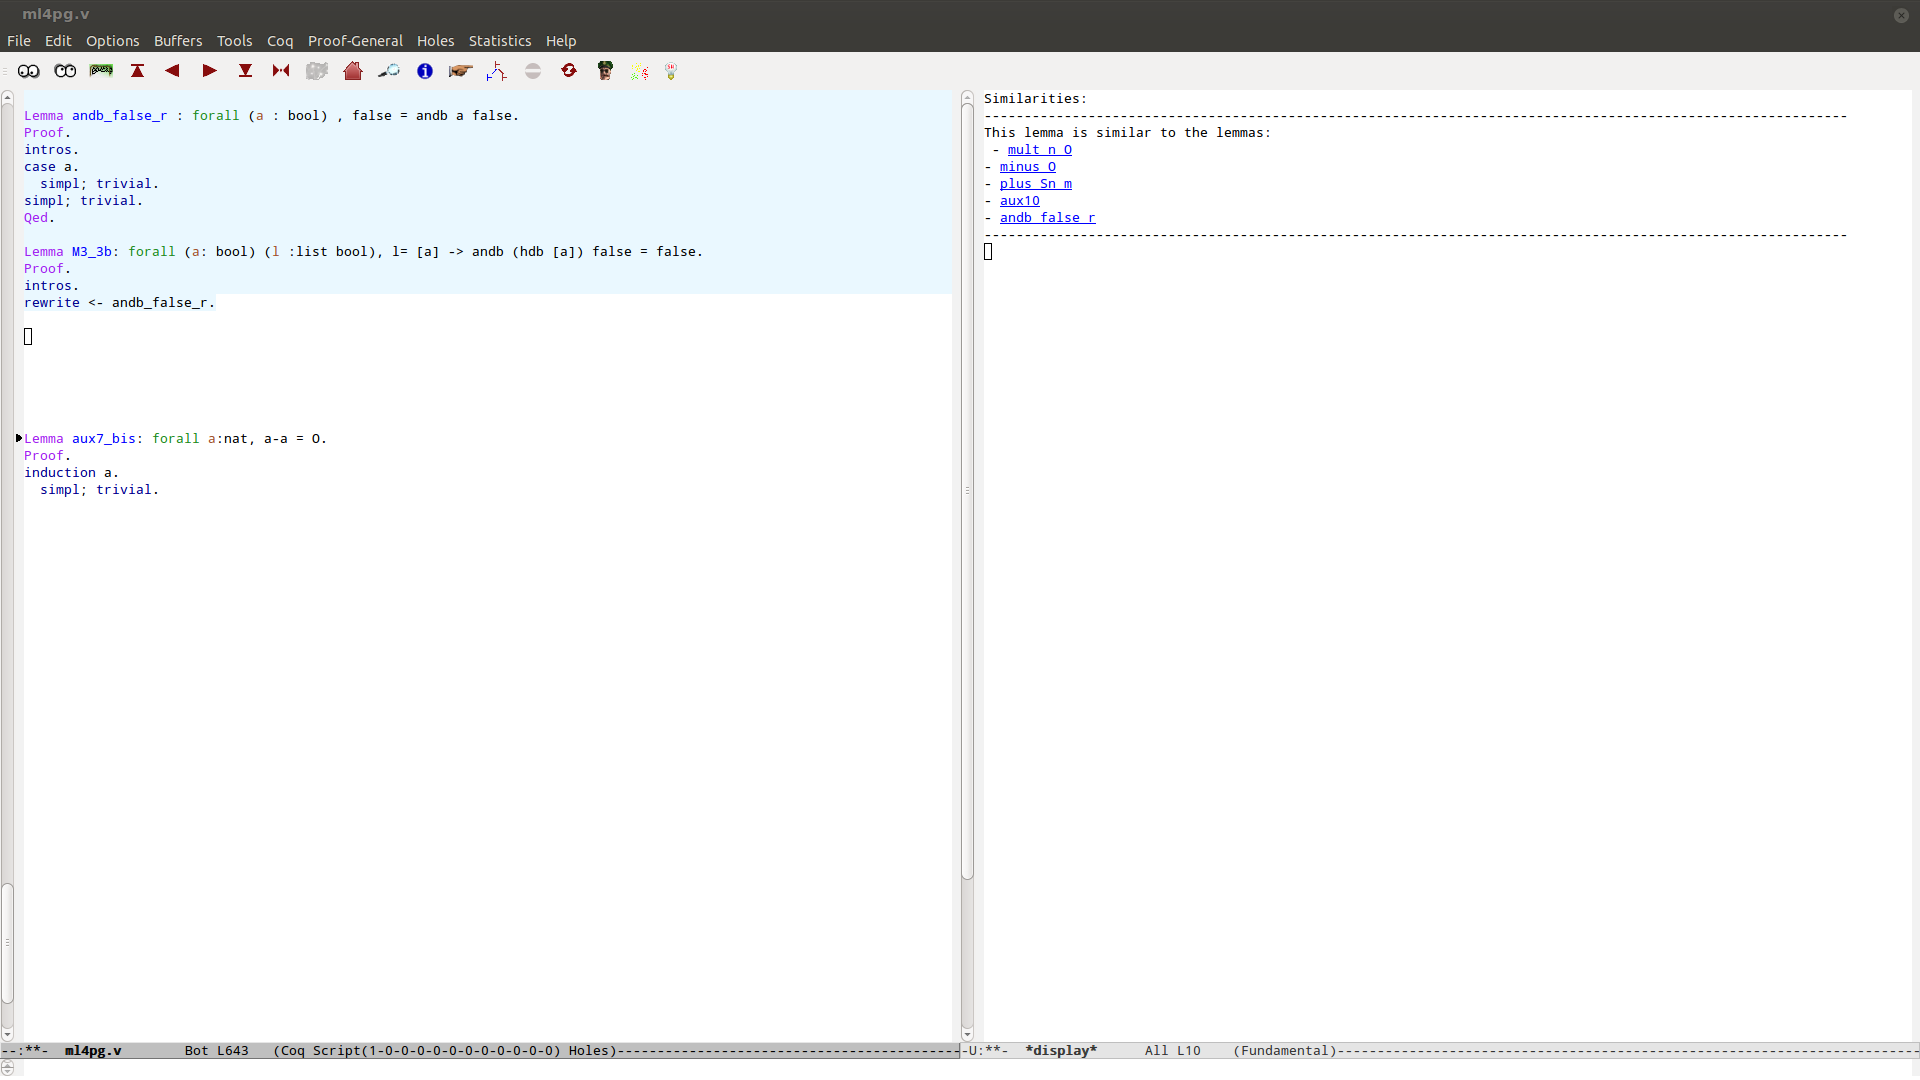
\includegraphics[scale=0.23]{images/clusters2pg.png}
 \caption{On the right side, several suggestions provided by ML4PG. If the user clicks on the name of one of the
suggested lemmas, a brief description about it is shown.}\label{clusters2}
\end{figure}

This functionality can also invoked using the right most button of the Proof General toolbar.

\subsection{Export Library}

Using the Export library option, the user can export the library for further use (see Figure~\ref{export}) with the 
Available libraries for clustering option. 


\begin{figure}
 \centering
 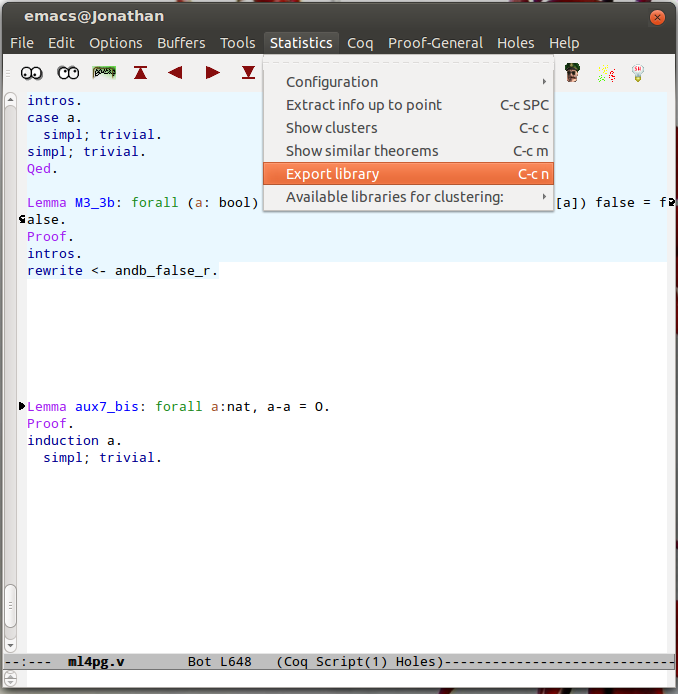
\includegraphics[scale=0.4]{images/export.png}
 \caption{ML4PG export menu.}\label{export}
\end{figure}








 
 
\bibliographystyle{plain} 
\bibliography{ml4pg_manual}

 
\end{document}
